\clearpage
\onecolumn
\section{Frontier Model and Case Atlas}
All 48 pairs are constructed evaluator controls, not model predictions. Field-answer images are context only.
Only the exported public JSON is allowed evidence; the plates do not define an image-only track.
\clearpage
\subsection{Courtyard Museum}
192 parts; 7 bottom-Y levels; dependency depth 7.
\subsubsection*{service plan}
\noindent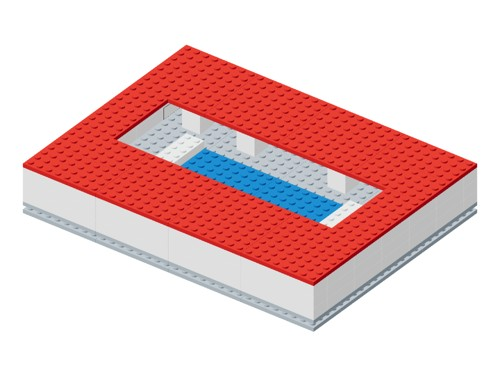
\includegraphics[width=.24\textwidth]{figures/frontier/courtyard-museum-service-plan-good.jpg}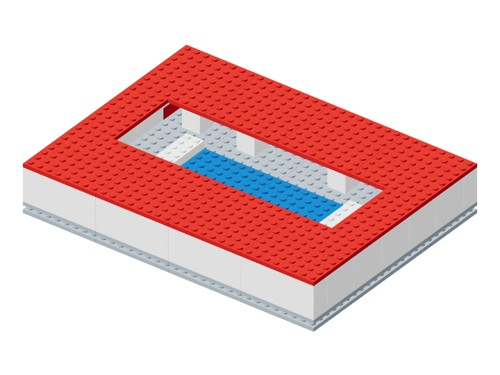
\includegraphics[width=.24\textwidth]{figures/frontier/courtyard-museum-service-plan-bad.jpg}\hfill\begin{minipage}[b]{.48\textwidth}\small Positive success: 1. Negative success: 0.\\Rejection: \texttt{blocked}.\\
Positive metrics: actions=10, lowerBound=10, finalExact=1, legalPrefix=1, excessActions=0.\end{minipage}\par
\subsubsection*{access certificate}
\noindent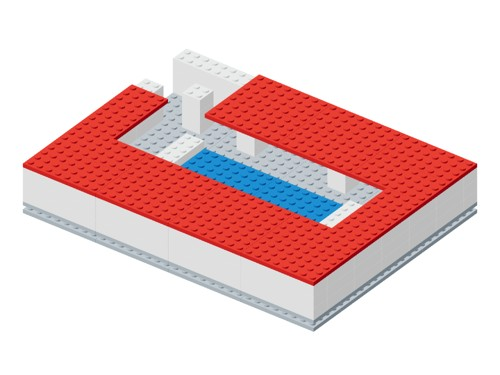
\includegraphics[width=.24\textwidth]{figures/frontier/courtyard-museum-access-certificate-good.jpg}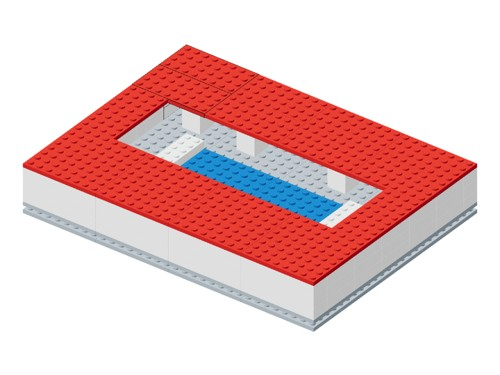
\includegraphics[width=.24\textwidth]{figures/frontier/courtyard-museum-access-certificate-bad.jpg}\hfill\begin{minipage}[b]{.48\textwidth}\small Positive success: 1. Negative success: 0.\\Rejection: \texttt{minimum\_set}.\\
Positive metrics: removals=5.\end{minipage}\par
\subsubsection*{parallel schedule}
\noindent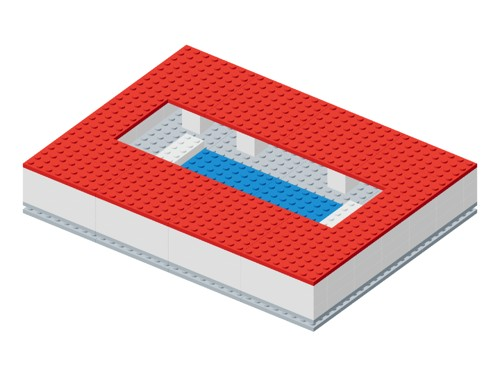
\includegraphics[width=.24\textwidth]{figures/frontier/courtyard-museum-parallel-schedule-good.jpg}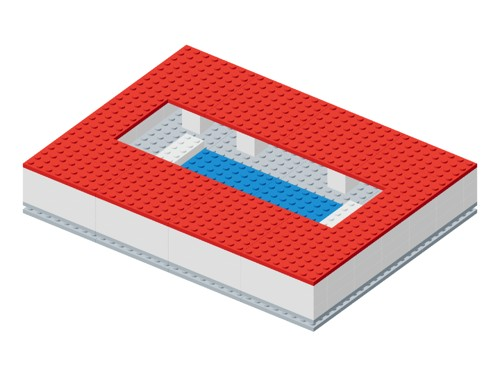
\includegraphics[width=.24\textwidth]{figures/frontier/courtyard-museum-parallel-schedule-bad.jpg}\hfill\begin{minipage}[b]{.48\textwidth}\small Positive success: 1. Negative success: 0.\\Rejection: \texttt{batch\_schema}.\\
Positive metrics: coverage=1, makespan=48, workerLowerBound=48.\end{minipage}\par
\subsubsection*{minimal intervention}
\noindent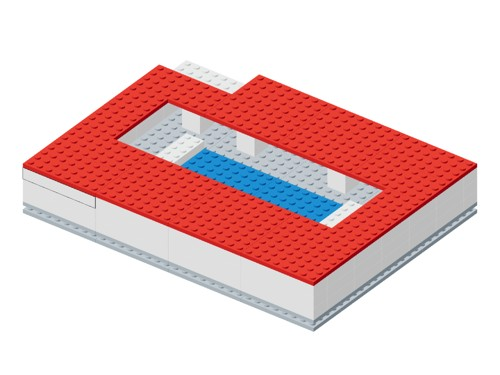
\includegraphics[width=.24\textwidth]{figures/frontier/courtyard-museum-minimal-intervention-good.jpg}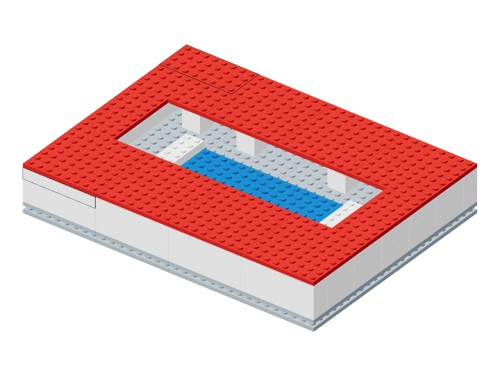
\includegraphics[width=.24\textwidth]{figures/frontier/courtyard-museum-minimal-intervention-bad.jpg}\hfill\begin{minipage}[b]{.48\textwidth}\small Positive success: 1. Negative success: 0.\\Rejection: \texttt{goal\_survives}.\\
Positive metrics: removals=2, optimum=2.\end{minipage}\par
\noindent\small\texttt{Positive: \{"removeIds": ["p0123", "p0131"], "cascadeIds": ["p0123", "p0131", "p0165"]\}}\par\normalsize
\clearpage
\subsection{Courtyard Museum (continued)}
192 parts; 7 bottom-Y levels; dependency depth 7.
\subsubsection*{inventory cover}
\noindent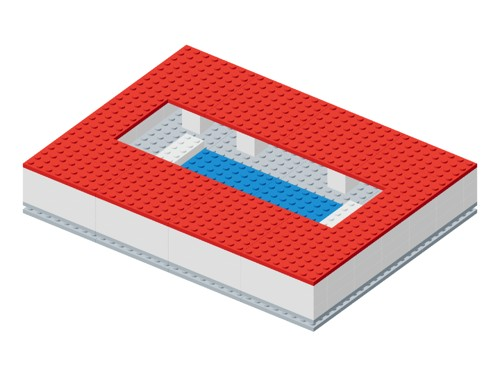
\includegraphics[width=.24\textwidth]{figures/frontier/courtyard-museum-inventory-cover-good.jpg}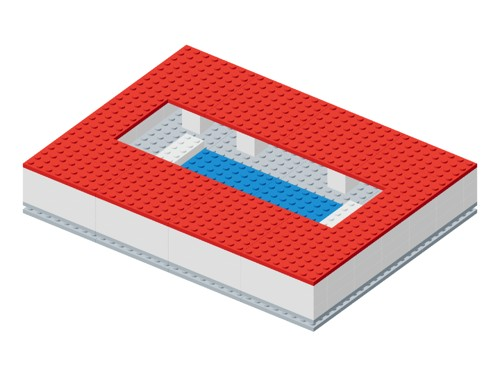
\includegraphics[width=.24\textwidth]{figures/frontier/courtyard-museum-inventory-cover-bad.jpg}\hfill\begin{minipage}[b]{.48\textwidth}\small Positive success: 1. Negative success: 0.\\Rejection: \texttt{uncovered}.\\
Positive metrics: coverage=1, tiles=7, lowerBound=7.\end{minipage}\par
\subsubsection*{ambiguity set}
\noindent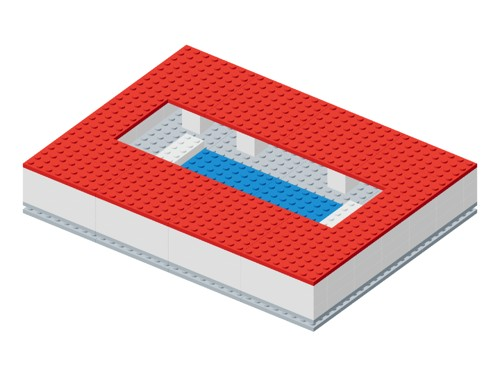
\includegraphics[width=.24\textwidth]{figures/frontier/courtyard-museum-ambiguity-set-good.jpg}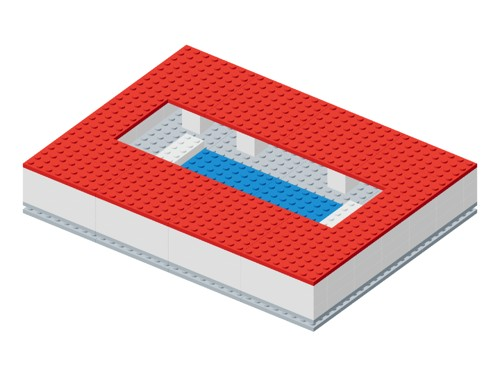
\includegraphics[width=.24\textwidth]{figures/frontier/courtyard-museum-ambiguity-set-bad.jpg}\hfill\begin{minipage}[b]{.48\textwidth}\small Positive success: 1. Negative success: 0.\\Rejection: \texttt{admissible\_set}.\\
Positive metrics: admissible=4, falseCertainty=0.\end{minipage}\par
\noindent\small\texttt{Positive: \{"possibleIds": ["h0", "h2", "h4", "h6"]\}}\par\normalsize
\subsubsection*{inspection policy}
\noindent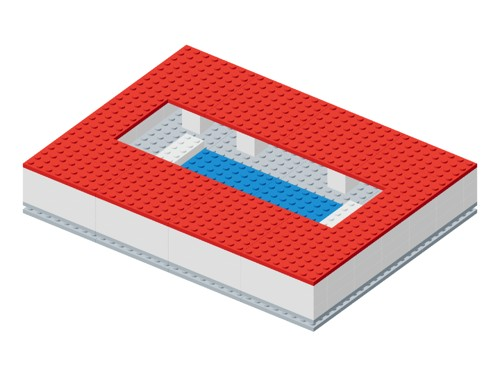
\includegraphics[width=.24\textwidth]{figures/frontier/courtyard-museum-inspection-policy-good.jpg}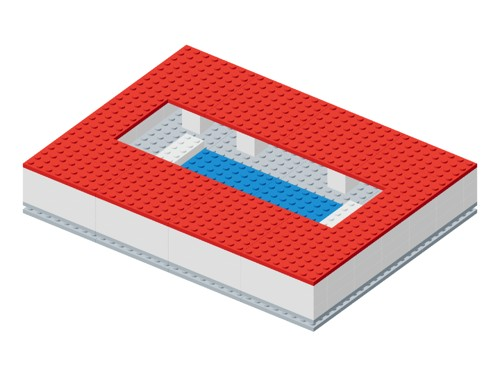
\includegraphics[width=.24\textwidth]{figures/frontier/courtyard-museum-inspection-policy-bad.jpg}\hfill\begin{minipage}[b]{.48\textwidth}\small Positive success: 1. Negative success: 0.\\Rejection: \texttt{policy\_coverage\_or\_budget}.\\
Positive metrics: worldCoverage=1, worstCost=6.\end{minipage}\par
\noindent\small Positive policy queries q0, q1, q2 and identifies all eight worlds at worst cost 6; the negative guesses h0 without querying. Full branch tree is in the corresponding review JSON.\par\normalsize
\subsubsection*{distributed repair}
\noindent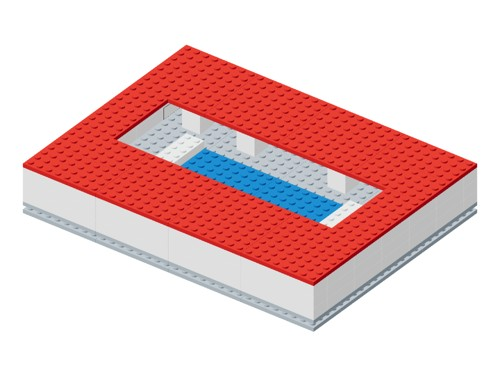
\includegraphics[width=.24\textwidth]{figures/frontier/courtyard-museum-distributed-repair-good.jpg}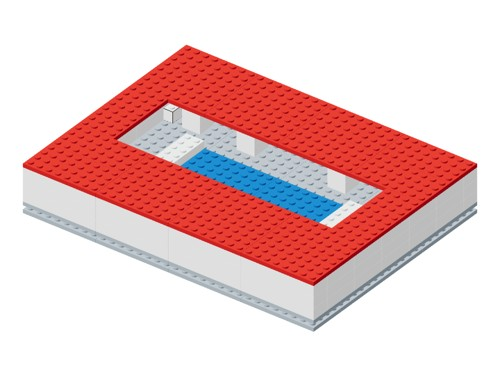
\includegraphics[width=.24\textwidth]{figures/frontier/courtyard-museum-distributed-repair-bad.jpg}\hfill\begin{minipage}[b]{.48\textwidth}\small Positive success: 1. Negative success: 0.\\Rejection: \texttt{fault\_set}.\\
Positive metrics: finalExact=1, changedRecall=1.\end{minipage}\par
\clearpage
\subsection{Intercity Terminal}
227 parts; 14 bottom-Y levels; dependency depth 14.
\subsubsection*{service plan}
\noindent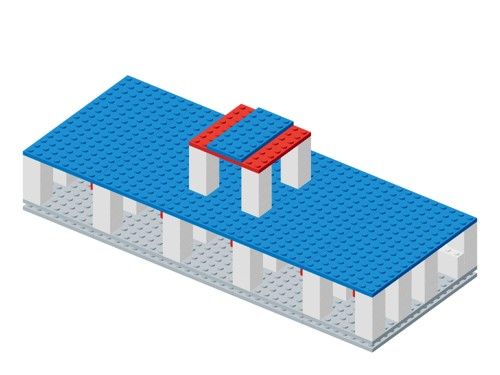
\includegraphics[width=.24\textwidth]{figures/frontier/intercity-terminal-service-plan-good.jpg}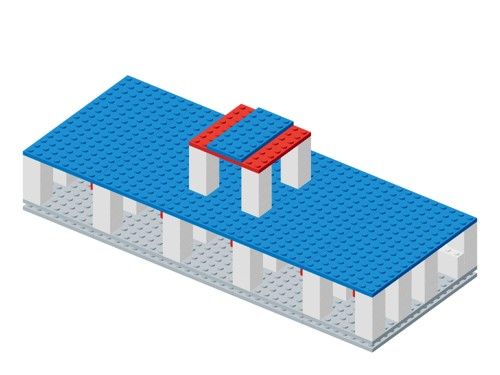
\includegraphics[width=.24\textwidth]{figures/frontier/intercity-terminal-service-plan-bad.jpg}\hfill\begin{minipage}[b]{.48\textwidth}\small Positive success: 1. Negative success: 0.\\Rejection: \texttt{blocked}.\\
Positive metrics: actions=30, lowerBound=30, finalExact=1, legalPrefix=1, excessActions=0.\end{minipage}\par
\subsubsection*{access certificate}
\noindent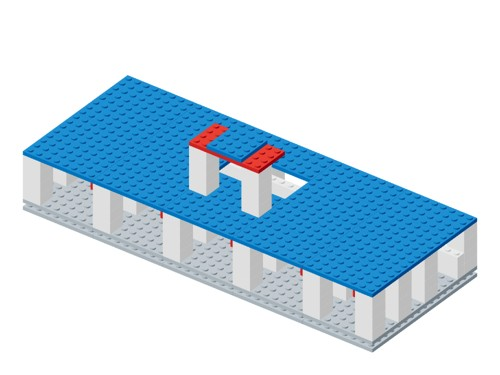
\includegraphics[width=.24\textwidth]{figures/frontier/intercity-terminal-access-certificate-good.jpg}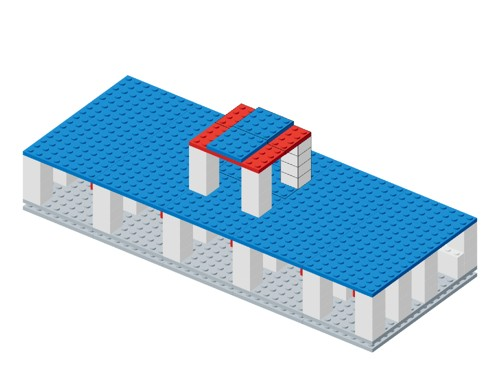
\includegraphics[width=.24\textwidth]{figures/frontier/intercity-terminal-access-certificate-bad.jpg}\hfill\begin{minipage}[b]{.48\textwidth}\small Positive success: 1. Negative success: 0.\\Rejection: \texttt{minimum\_set}.\\
Positive metrics: removals=15.\end{minipage}\par
\subsubsection*{parallel schedule}
\noindent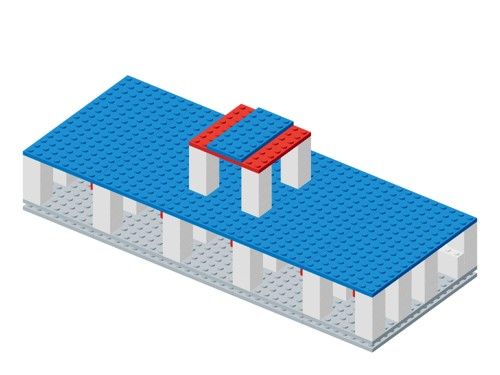
\includegraphics[width=.24\textwidth]{figures/frontier/intercity-terminal-parallel-schedule-good.jpg}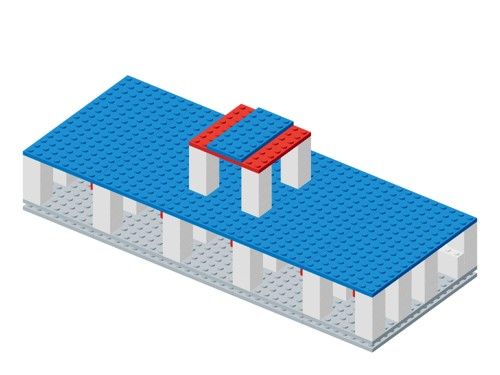
\includegraphics[width=.24\textwidth]{figures/frontier/intercity-terminal-parallel-schedule-bad.jpg}\hfill\begin{minipage}[b]{.48\textwidth}\small Positive success: 1. Negative success: 0.\\Rejection: \texttt{batch\_schema}.\\
Positive metrics: coverage=1, makespan=58, workerLowerBound=57.\end{minipage}\par
\subsubsection*{minimal intervention}
\noindent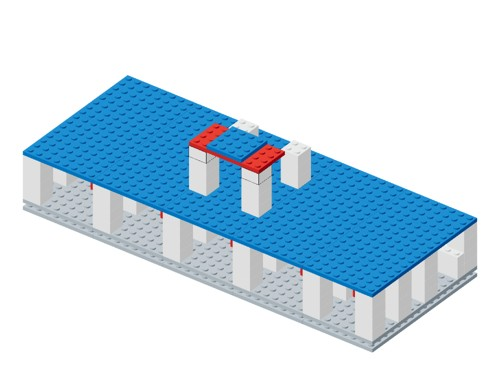
\includegraphics[width=.24\textwidth]{figures/frontier/intercity-terminal-minimal-intervention-good.jpg}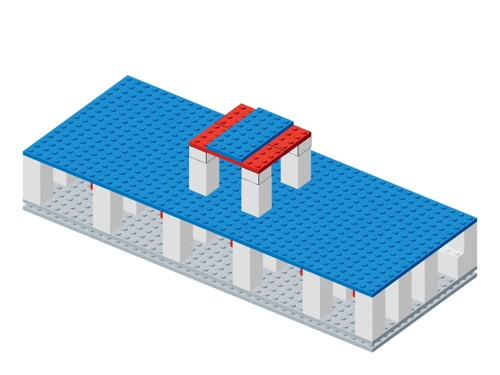
\includegraphics[width=.24\textwidth]{figures/frontier/intercity-terminal-minimal-intervention-bad.jpg}\hfill\begin{minipage}[b]{.48\textwidth}\small Positive success: 1. Negative success: 0.\\Rejection: \texttt{goal\_survives}.\\
Positive metrics: removals=2, optimum=2.\end{minipage}\par
\noindent\small\texttt{Positive: \{"removeIds": ["p0211", "p0219"], "cascadeIds": ["p0211", "p0219", "p0224", "p0226"]\}}\par\normalsize
\clearpage
\subsection{Intercity Terminal (continued)}
227 parts; 14 bottom-Y levels; dependency depth 14.
\subsubsection*{inventory cover}
\noindent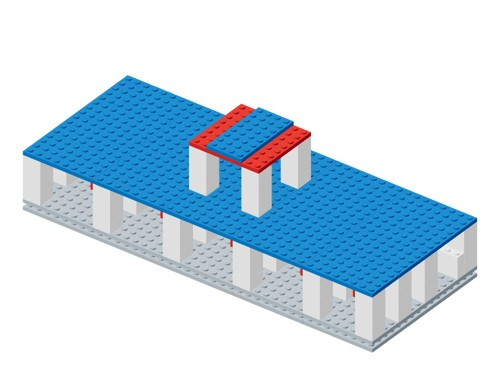
\includegraphics[width=.24\textwidth]{figures/frontier/intercity-terminal-inventory-cover-good.jpg}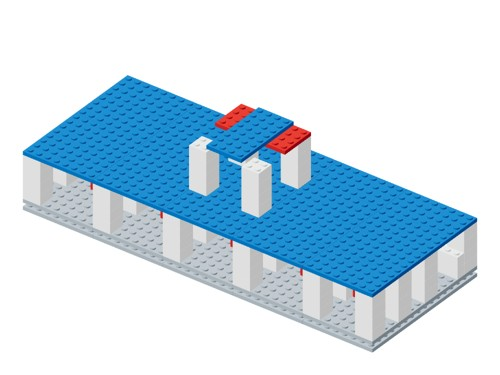
\includegraphics[width=.24\textwidth]{figures/frontier/intercity-terminal-inventory-cover-bad.jpg}\hfill\begin{minipage}[b]{.48\textwidth}\small Positive success: 1. Negative success: 0.\\Rejection: \texttt{uncovered}.\\
Positive metrics: coverage=1, tiles=5, lowerBound=5.\end{minipage}\par
\subsubsection*{ambiguity set}
\noindent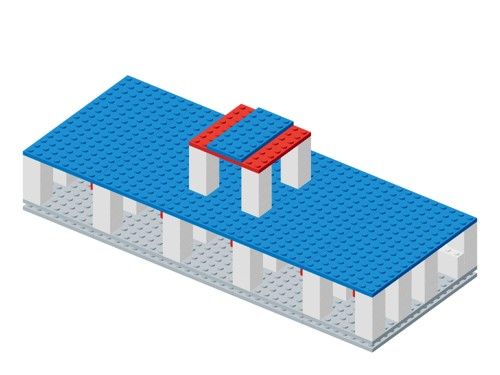
\includegraphics[width=.24\textwidth]{figures/frontier/intercity-terminal-ambiguity-set-good.jpg}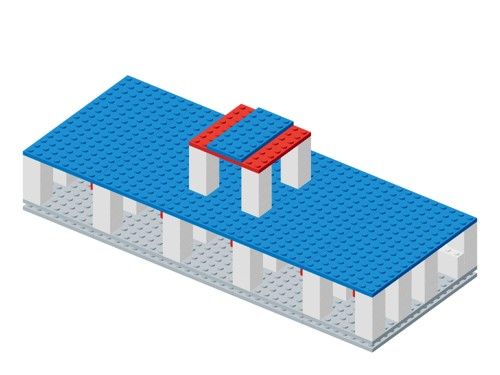
\includegraphics[width=.24\textwidth]{figures/frontier/intercity-terminal-ambiguity-set-bad.jpg}\hfill\begin{minipage}[b]{.48\textwidth}\small Positive success: 1. Negative success: 0.\\Rejection: \texttt{admissible\_set}.\\
Positive metrics: admissible=4, falseCertainty=0.\end{minipage}\par
\noindent\small\texttt{Positive: \{"possibleIds": ["h0", "h2", "h4", "h6"]\}}\par\normalsize
\subsubsection*{inspection policy}
\noindent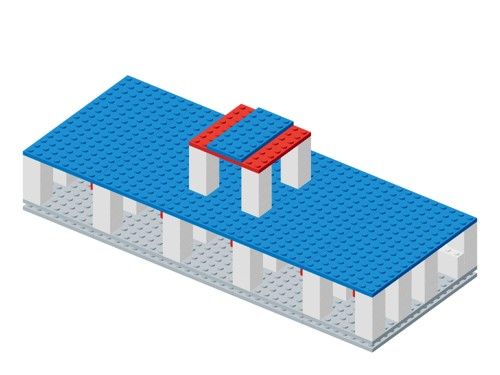
\includegraphics[width=.24\textwidth]{figures/frontier/intercity-terminal-inspection-policy-good.jpg}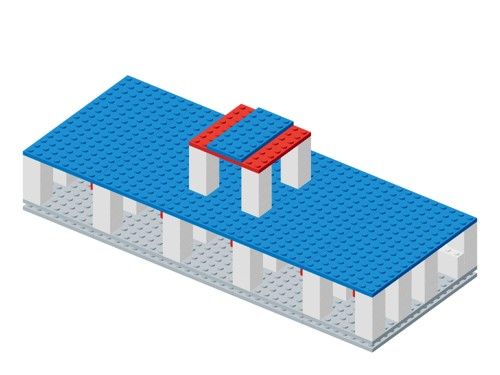
\includegraphics[width=.24\textwidth]{figures/frontier/intercity-terminal-inspection-policy-bad.jpg}\hfill\begin{minipage}[b]{.48\textwidth}\small Positive success: 1. Negative success: 0.\\Rejection: \texttt{policy\_coverage\_or\_budget}.\\
Positive metrics: worldCoverage=1, worstCost=6.\end{minipage}\par
\noindent\small Positive policy queries q0, q1, q2 and identifies all eight worlds at worst cost 6; the negative guesses h0 without querying. Full branch tree is in the corresponding review JSON.\par\normalsize
\subsubsection*{distributed repair}
\noindent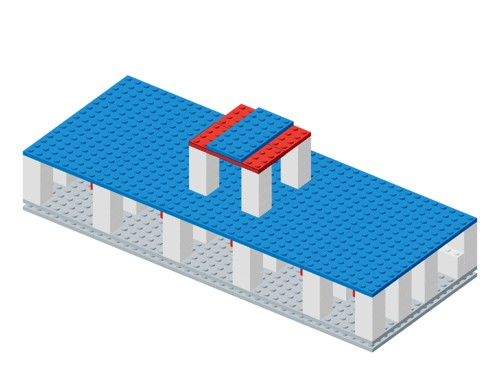
\includegraphics[width=.24\textwidth]{figures/frontier/intercity-terminal-distributed-repair-good.jpg}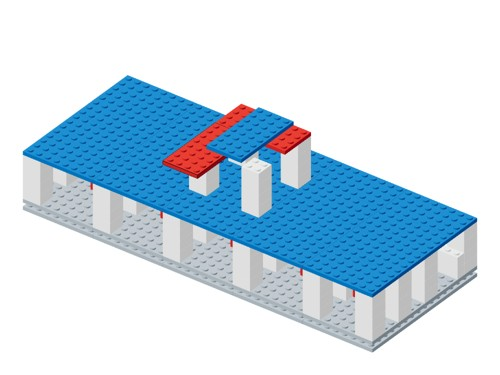
\includegraphics[width=.24\textwidth]{figures/frontier/intercity-terminal-distributed-repair-bad.jpg}\hfill\begin{minipage}[b]{.48\textwidth}\small Positive success: 1. Negative success: 0.\\Rejection: \texttt{fault\_set}.\\
Positive metrics: finalExact=1, changedRecall=1.\end{minipage}\par
\clearpage
\subsection{Coastal Cargo Vessel}
158 parts; 11 bottom-Y levels; dependency depth 11.
\subsubsection*{service plan}
\noindent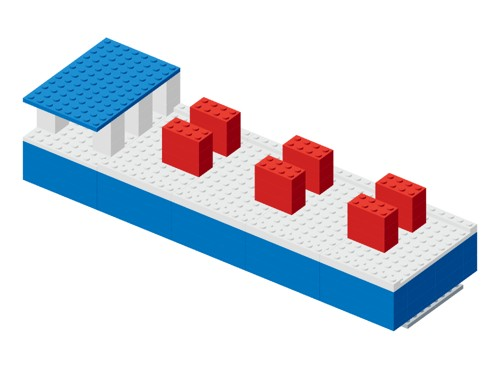
\includegraphics[width=.24\textwidth]{figures/frontier/coastal-cargo-vessel-service-plan-good.jpg}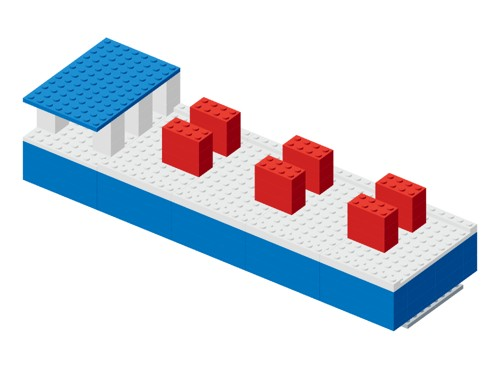
\includegraphics[width=.24\textwidth]{figures/frontier/coastal-cargo-vessel-service-plan-bad.jpg}\hfill\begin{minipage}[b]{.48\textwidth}\small Positive success: 1. Negative success: 0.\\Rejection: \texttt{blocked}.\\
Positive metrics: actions=38, lowerBound=38, finalExact=1, legalPrefix=1, excessActions=0.\end{minipage}\par
\subsubsection*{access certificate}
\noindent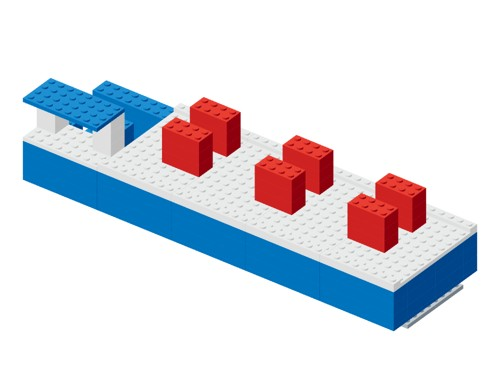
\includegraphics[width=.24\textwidth]{figures/frontier/coastal-cargo-vessel-access-certificate-good.jpg}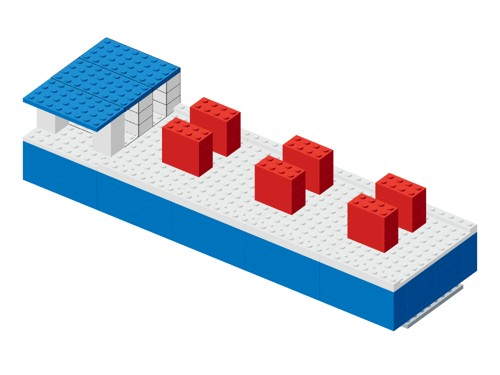
\includegraphics[width=.24\textwidth]{figures/frontier/coastal-cargo-vessel-access-certificate-bad.jpg}\hfill\begin{minipage}[b]{.48\textwidth}\small Positive success: 1. Negative success: 0.\\Rejection: \texttt{minimum\_set}.\\
Positive metrics: removals=19.\end{minipage}\par
\subsubsection*{parallel schedule}
\noindent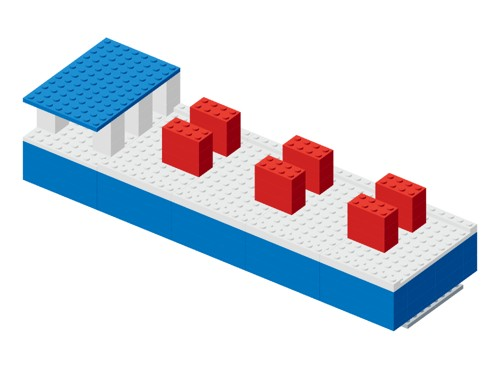
\includegraphics[width=.24\textwidth]{figures/frontier/coastal-cargo-vessel-parallel-schedule-good.jpg}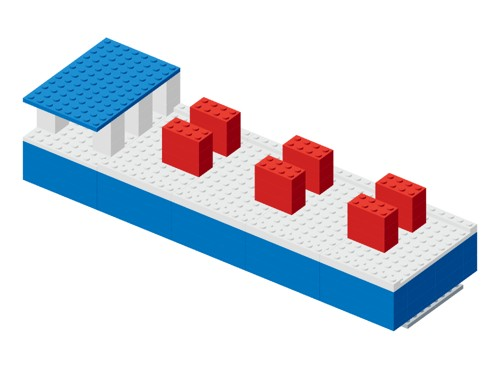
\includegraphics[width=.24\textwidth]{figures/frontier/coastal-cargo-vessel-parallel-schedule-bad.jpg}\hfill\begin{minipage}[b]{.48\textwidth}\small Positive success: 1. Negative success: 0.\\Rejection: \texttt{batch\_schema}.\\
Positive metrics: coverage=1, makespan=40, workerLowerBound=40.\end{minipage}\par
\subsubsection*{minimal intervention}
\noindent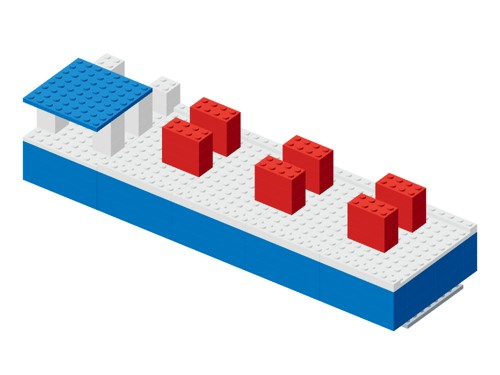
\includegraphics[width=.24\textwidth]{figures/frontier/coastal-cargo-vessel-minimal-intervention-good.jpg}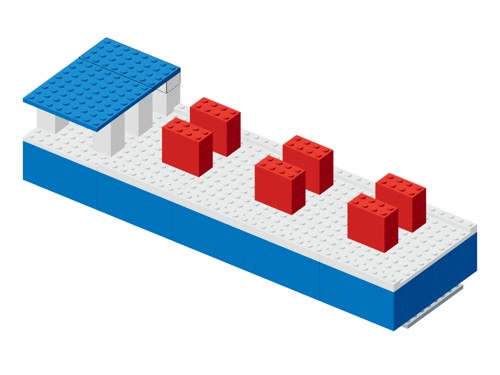
\includegraphics[width=.24\textwidth]{figures/frontier/coastal-cargo-vessel-minimal-intervention-bad.jpg}\hfill\begin{minipage}[b]{.48\textwidth}\small Positive success: 1. Negative success: 0.\\Rejection: \texttt{goal\_survives}.\\
Positive metrics: removals=2, optimum=2.\end{minipage}\par
\noindent\small\texttt{Positive: \{"removeIds": ["p0114", "p0123"], "cascadeIds": ["p0114", "p0123", "p0130"]\}}\par\normalsize
\clearpage
\subsection{Coastal Cargo Vessel (continued)}
158 parts; 11 bottom-Y levels; dependency depth 11.
\subsubsection*{inventory cover}
\noindent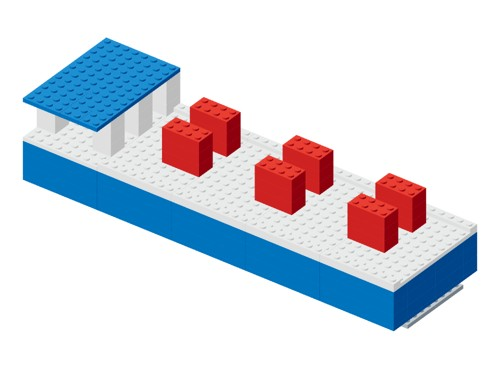
\includegraphics[width=.24\textwidth]{figures/frontier/coastal-cargo-vessel-inventory-cover-good.jpg}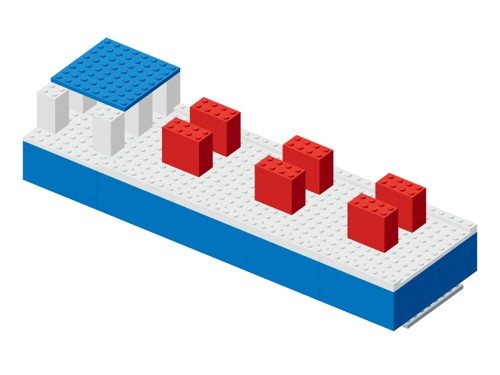
\includegraphics[width=.24\textwidth]{figures/frontier/coastal-cargo-vessel-inventory-cover-bad.jpg}\hfill\begin{minipage}[b]{.48\textwidth}\small Positive success: 1. Negative success: 0.\\Rejection: \texttt{uncovered}.\\
Positive metrics: coverage=1, tiles=5, lowerBound=5.\end{minipage}\par
\subsubsection*{ambiguity set}
\noindent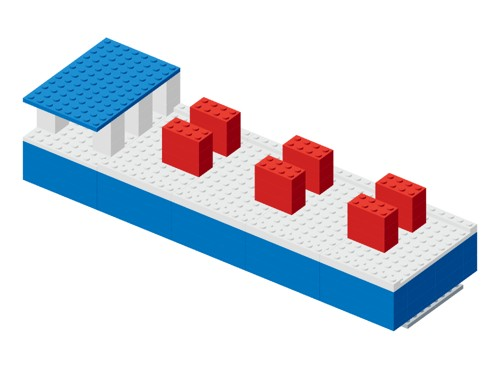
\includegraphics[width=.24\textwidth]{figures/frontier/coastal-cargo-vessel-ambiguity-set-good.jpg}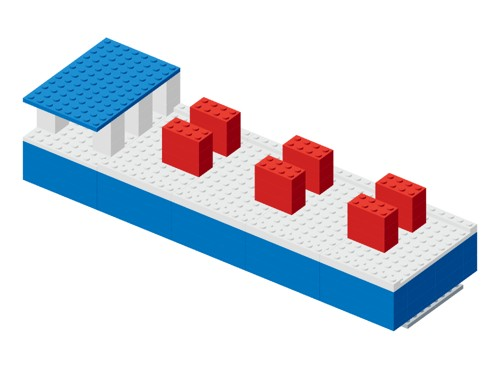
\includegraphics[width=.24\textwidth]{figures/frontier/coastal-cargo-vessel-ambiguity-set-bad.jpg}\hfill\begin{minipage}[b]{.48\textwidth}\small Positive success: 1. Negative success: 0.\\Rejection: \texttt{admissible\_set}.\\
Positive metrics: admissible=4, falseCertainty=0.\end{minipage}\par
\noindent\small\texttt{Positive: \{"possibleIds": ["h0", "h2", "h4", "h6"]\}}\par\normalsize
\subsubsection*{inspection policy}
\noindent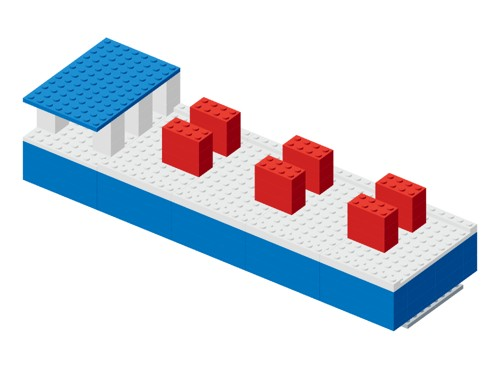
\includegraphics[width=.24\textwidth]{figures/frontier/coastal-cargo-vessel-inspection-policy-good.jpg}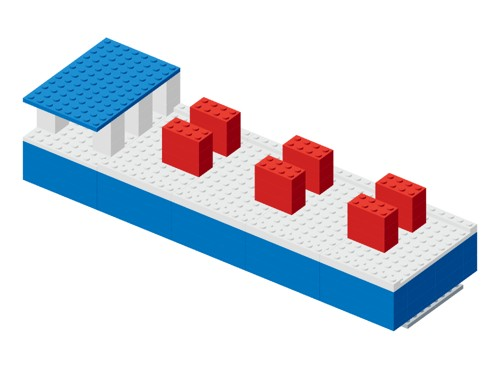
\includegraphics[width=.24\textwidth]{figures/frontier/coastal-cargo-vessel-inspection-policy-bad.jpg}\hfill\begin{minipage}[b]{.48\textwidth}\small Positive success: 1. Negative success: 0.\\Rejection: \texttt{policy\_coverage\_or\_budget}.\\
Positive metrics: worldCoverage=1, worstCost=6.\end{minipage}\par
\noindent\small Positive policy queries q0, q1, q2 and identifies all eight worlds at worst cost 6; the negative guesses h0 without querying. Full branch tree is in the corresponding review JSON.\par\normalsize
\subsubsection*{distributed repair}
\noindent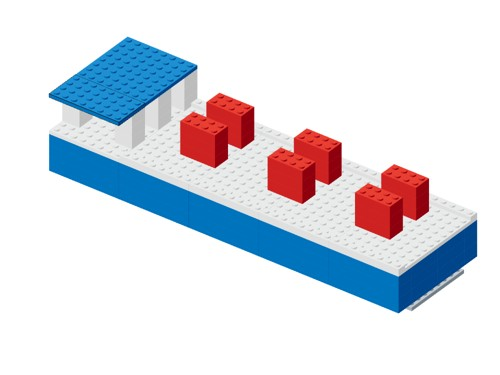
\includegraphics[width=.24\textwidth]{figures/frontier/coastal-cargo-vessel-distributed-repair-good.jpg}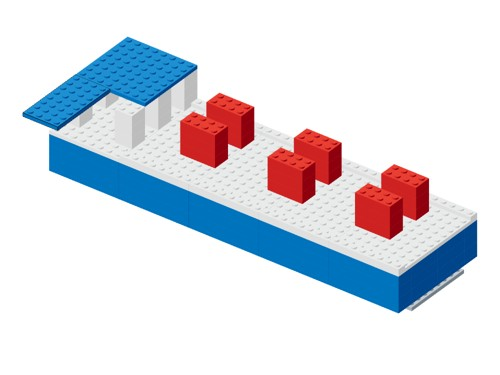
\includegraphics[width=.24\textwidth]{figures/frontier/coastal-cargo-vessel-distributed-repair-bad.jpg}\hfill\begin{minipage}[b]{.48\textwidth}\small Positive success: 1. Negative success: 0.\\Rejection: \texttt{fault\_set}.\\
Positive metrics: finalExact=1, changedRecall=1.\end{minipage}\par
\clearpage
\subsection{Four-Tower Citadel}
236 parts; 11 bottom-Y levels; dependency depth 11.
\subsubsection*{service plan}
\noindent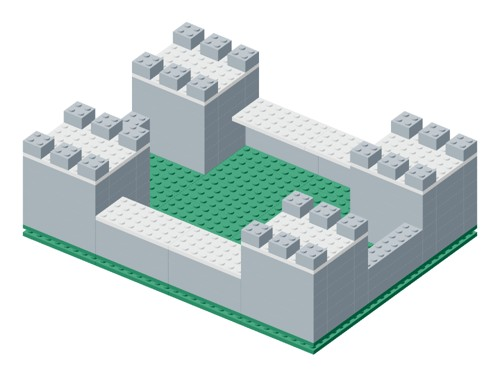
\includegraphics[width=.24\textwidth]{figures/frontier/four-tower-citadel-service-plan-good.jpg}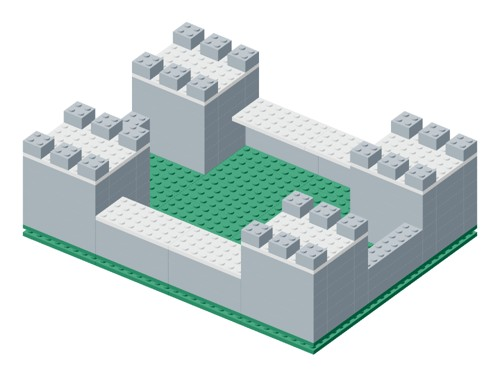
\includegraphics[width=.24\textwidth]{figures/frontier/four-tower-citadel-service-plan-bad.jpg}\hfill\begin{minipage}[b]{.48\textwidth}\small Positive success: 1. Negative success: 0.\\Rejection: \texttt{blocked}.\\
Positive metrics: actions=28, lowerBound=28, finalExact=1, legalPrefix=1, excessActions=0.\end{minipage}\par
\subsubsection*{access certificate}
\noindent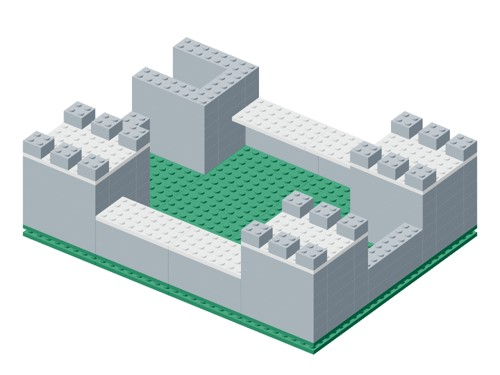
\includegraphics[width=.24\textwidth]{figures/frontier/four-tower-citadel-access-certificate-good.jpg}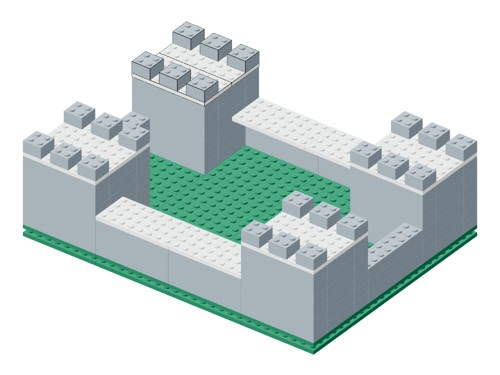
\includegraphics[width=.24\textwidth]{figures/frontier/four-tower-citadel-access-certificate-bad.jpg}\hfill\begin{minipage}[b]{.48\textwidth}\small Positive success: 1. Negative success: 0.\\Rejection: \texttt{minimum\_set}.\\
Positive metrics: removals=14.\end{minipage}\par
\subsubsection*{parallel schedule}
\noindent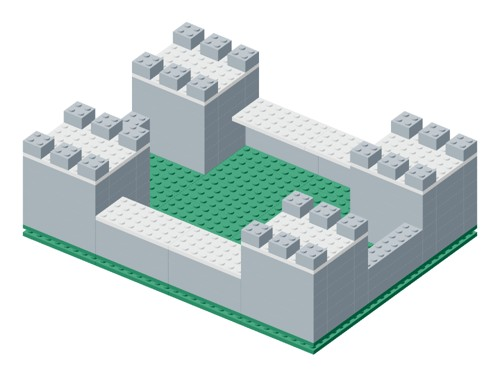
\includegraphics[width=.24\textwidth]{figures/frontier/four-tower-citadel-parallel-schedule-good.jpg}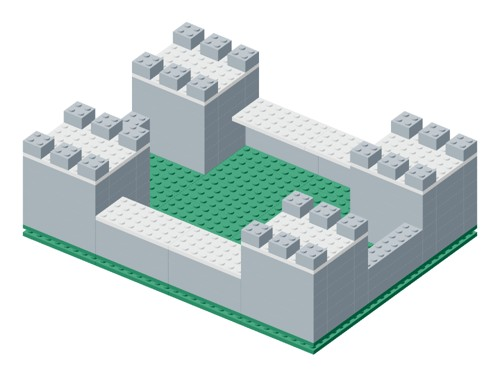
\includegraphics[width=.24\textwidth]{figures/frontier/four-tower-citadel-parallel-schedule-bad.jpg}\hfill\begin{minipage}[b]{.48\textwidth}\small Positive success: 1. Negative success: 0.\\Rejection: \texttt{batch\_schema}.\\
Positive metrics: coverage=1, makespan=59, workerLowerBound=59.\end{minipage}\par
\subsubsection*{minimal intervention}
\noindent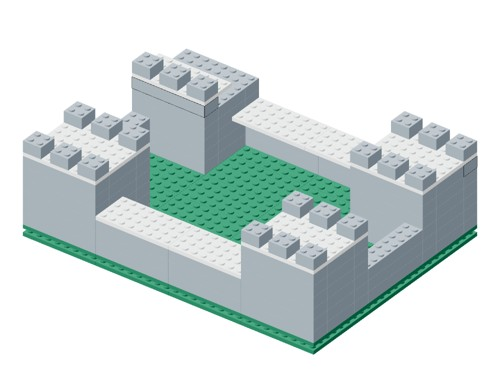
\includegraphics[width=.24\textwidth]{figures/frontier/four-tower-citadel-minimal-intervention-good.jpg}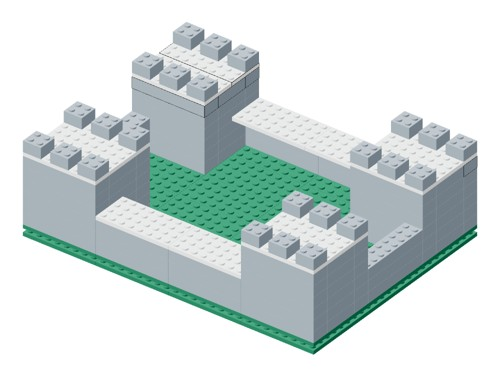
\includegraphics[width=.24\textwidth]{figures/frontier/four-tower-citadel-minimal-intervention-bad.jpg}\hfill\begin{minipage}[b]{.48\textwidth}\small Positive success: 1. Negative success: 0.\\Rejection: \texttt{goal\_survives}.\\
Positive metrics: removals=3, optimum=3.\end{minipage}\par
\noindent\small\texttt{Positive: \{"removeIds": ["p0107", "p0109", "p0110"], "cascadeIds": ["p0107", "p0109", "p0110", "p0111", "p0113", "p0115", "p0117"]\}}\par\normalsize
\clearpage
\subsection{Four-Tower Citadel (continued)}
236 parts; 11 bottom-Y levels; dependency depth 11.
\subsubsection*{inventory cover}
\noindent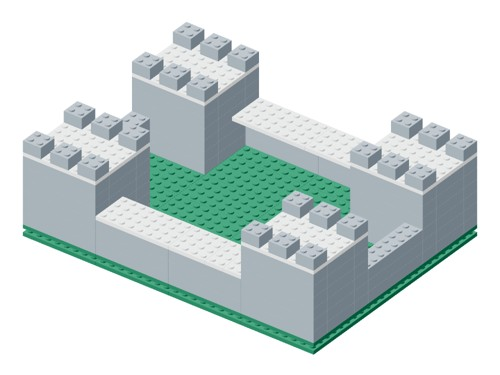
\includegraphics[width=.24\textwidth]{figures/frontier/four-tower-citadel-inventory-cover-good.jpg}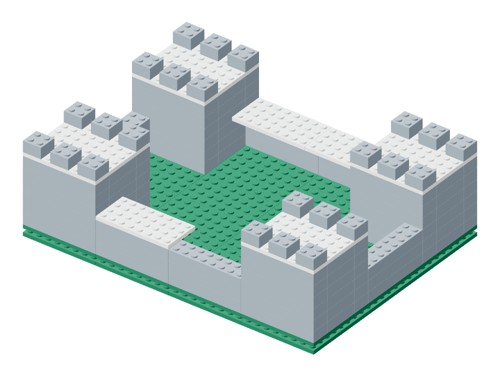
\includegraphics[width=.24\textwidth]{figures/frontier/four-tower-citadel-inventory-cover-bad.jpg}\hfill\begin{minipage}[b]{.48\textwidth}\small Positive success: 1. Negative success: 0.\\Rejection: \texttt{uncovered}.\\
Positive metrics: coverage=1, tiles=5, lowerBound=5.\end{minipage}\par
\subsubsection*{ambiguity set}
\noindent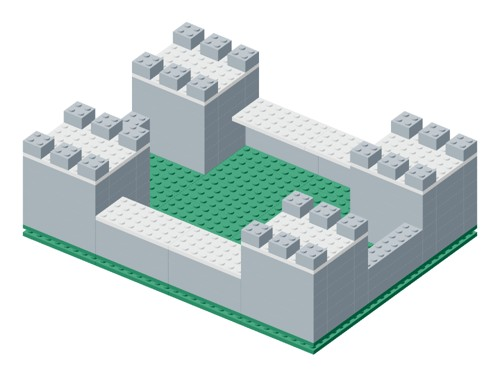
\includegraphics[width=.24\textwidth]{figures/frontier/four-tower-citadel-ambiguity-set-good.jpg}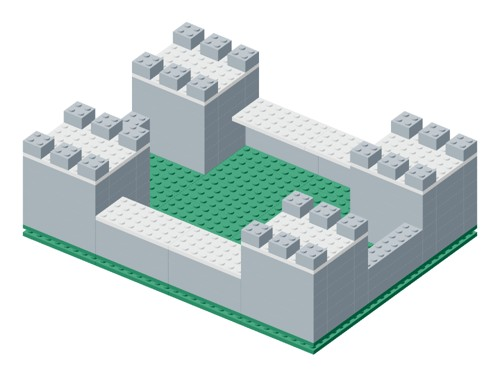
\includegraphics[width=.24\textwidth]{figures/frontier/four-tower-citadel-ambiguity-set-bad.jpg}\hfill\begin{minipage}[b]{.48\textwidth}\small Positive success: 1. Negative success: 0.\\Rejection: \texttt{admissible\_set}.\\
Positive metrics: admissible=4, falseCertainty=0.\end{minipage}\par
\noindent\small\texttt{Positive: \{"possibleIds": ["h0", "h2", "h4", "h6"]\}}\par\normalsize
\subsubsection*{inspection policy}
\noindent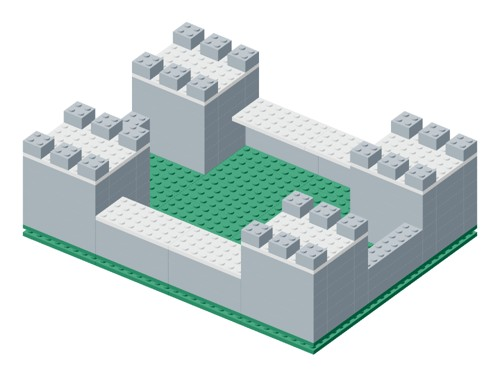
\includegraphics[width=.24\textwidth]{figures/frontier/four-tower-citadel-inspection-policy-good.jpg}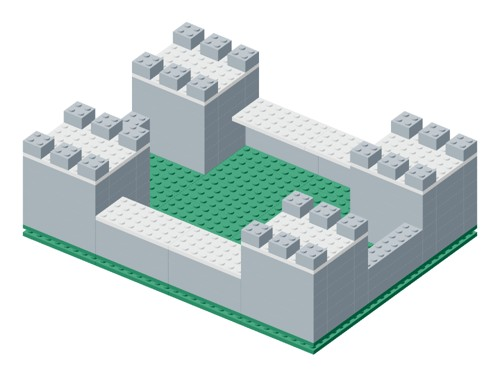
\includegraphics[width=.24\textwidth]{figures/frontier/four-tower-citadel-inspection-policy-bad.jpg}\hfill\begin{minipage}[b]{.48\textwidth}\small Positive success: 1. Negative success: 0.\\Rejection: \texttt{policy\_coverage\_or\_budget}.\\
Positive metrics: worldCoverage=1, worstCost=6.\end{minipage}\par
\noindent\small Positive policy queries q0, q1, q2 and identifies all eight worlds at worst cost 6; the negative guesses h0 without querying. Full branch tree is in the corresponding review JSON.\par\normalsize
\subsubsection*{distributed repair}
\noindent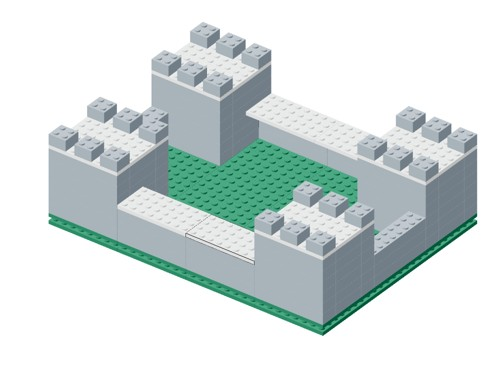
\includegraphics[width=.24\textwidth]{figures/frontier/four-tower-citadel-distributed-repair-good.jpg}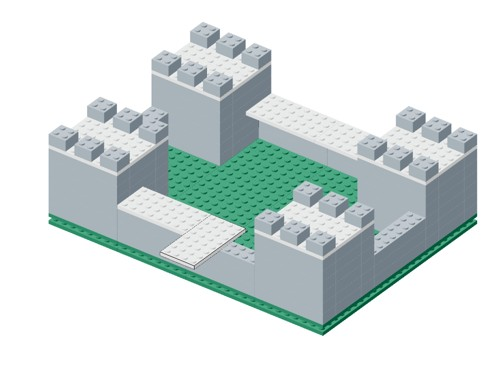
\includegraphics[width=.24\textwidth]{figures/frontier/four-tower-citadel-distributed-repair-bad.jpg}\hfill\begin{minipage}[b]{.48\textwidth}\small Positive success: 1. Negative success: 0.\\Rejection: \texttt{fault\_set}.\\
Positive metrics: finalExact=1, changedRecall=1.\end{minipage}\par
\clearpage
\subsection{Process Service Plant}
288 parts; 16 bottom-Y levels; dependency depth 14.
\subsubsection*{service plan}
\noindent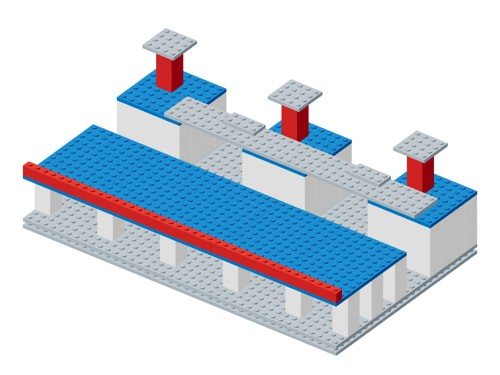
\includegraphics[width=.24\textwidth]{figures/frontier/process-service-plant-service-plan-good.jpg}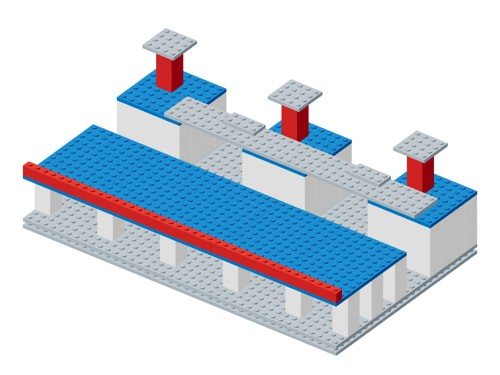
\includegraphics[width=.24\textwidth]{figures/frontier/process-service-plant-service-plan-bad.jpg}\hfill\begin{minipage}[b]{.48\textwidth}\small Positive success: 1. Negative success: 0.\\Rejection: \texttt{blocked}.\\
Positive metrics: actions=32, lowerBound=32, finalExact=1, legalPrefix=1, excessActions=0.\end{minipage}\par
\subsubsection*{access certificate}
\noindent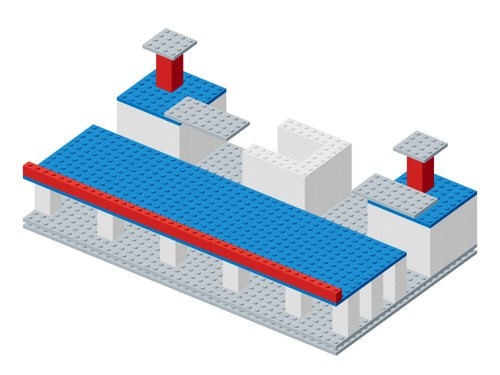
\includegraphics[width=.24\textwidth]{figures/frontier/process-service-plant-access-certificate-good.jpg}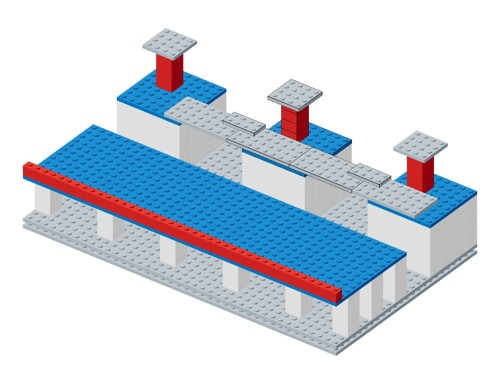
\includegraphics[width=.24\textwidth]{figures/frontier/process-service-plant-access-certificate-bad.jpg}\hfill\begin{minipage}[b]{.48\textwidth}\small Positive success: 1. Negative success: 0.\\Rejection: \texttt{minimum\_set}.\\
Positive metrics: removals=16.\end{minipage}\par
\subsubsection*{parallel schedule}
\noindent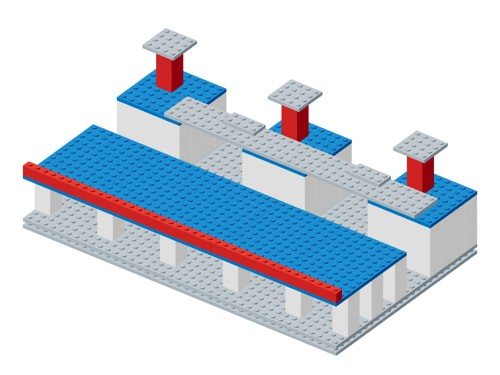
\includegraphics[width=.24\textwidth]{figures/frontier/process-service-plant-parallel-schedule-good.jpg}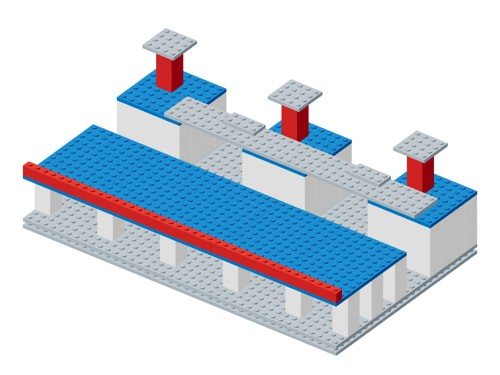
\includegraphics[width=.24\textwidth]{figures/frontier/process-service-plant-parallel-schedule-bad.jpg}\hfill\begin{minipage}[b]{.48\textwidth}\small Positive success: 1. Negative success: 0.\\Rejection: \texttt{batch\_schema}.\\
Positive metrics: coverage=1, makespan=73, workerLowerBound=72.\end{minipage}\par
\subsubsection*{minimal intervention}
\noindent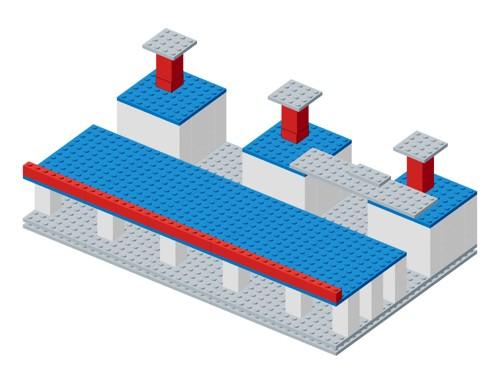
\includegraphics[width=.24\textwidth]{figures/frontier/process-service-plant-minimal-intervention-good.jpg}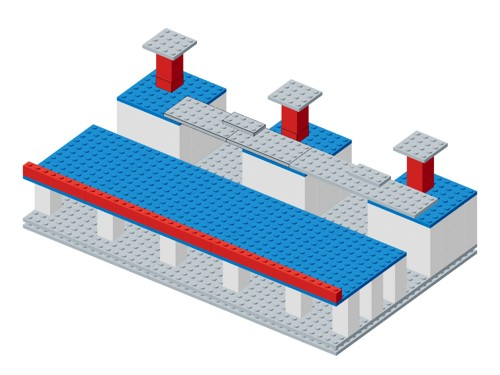
\includegraphics[width=.24\textwidth]{figures/frontier/process-service-plant-minimal-intervention-bad.jpg}\hfill\begin{minipage}[b]{.48\textwidth}\small Positive success: 1. Negative success: 0.\\Rejection: \texttt{goal\_survives}.\\
Positive metrics: removals=2, optimum=2.\end{minipage}\par
\noindent\small\texttt{Positive: \{"removeIds": ["p0283", "p0284"], "cascadeIds": ["p0283", "p0284", "p0285"]\}}\par\normalsize
\clearpage
\subsection{Process Service Plant (continued)}
288 parts; 16 bottom-Y levels; dependency depth 14.
\subsubsection*{inventory cover}
\noindent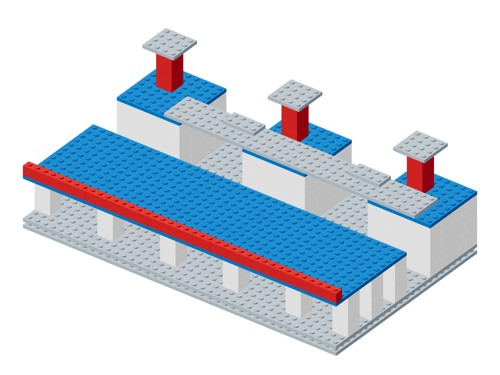
\includegraphics[width=.24\textwidth]{figures/frontier/process-service-plant-inventory-cover-good.jpg}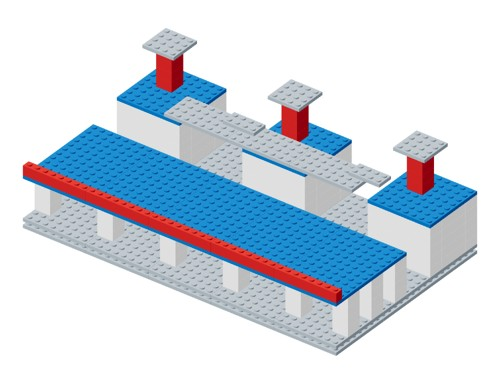
\includegraphics[width=.24\textwidth]{figures/frontier/process-service-plant-inventory-cover-bad.jpg}\hfill\begin{minipage}[b]{.48\textwidth}\small Positive success: 1. Negative success: 0.\\Rejection: \texttt{uncovered}.\\
Positive metrics: coverage=1, tiles=7, lowerBound=7.\end{minipage}\par
\subsubsection*{ambiguity set}
\noindent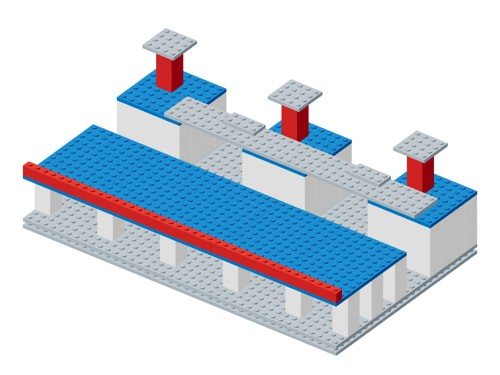
\includegraphics[width=.24\textwidth]{figures/frontier/process-service-plant-ambiguity-set-good.jpg}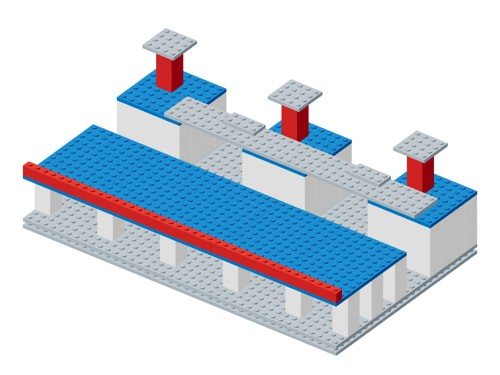
\includegraphics[width=.24\textwidth]{figures/frontier/process-service-plant-ambiguity-set-bad.jpg}\hfill\begin{minipage}[b]{.48\textwidth}\small Positive success: 1. Negative success: 0.\\Rejection: \texttt{admissible\_set}.\\
Positive metrics: admissible=4, falseCertainty=0.\end{minipage}\par
\noindent\small\texttt{Positive: \{"possibleIds": ["h0", "h2", "h4", "h6"]\}}\par\normalsize
\subsubsection*{inspection policy}
\noindent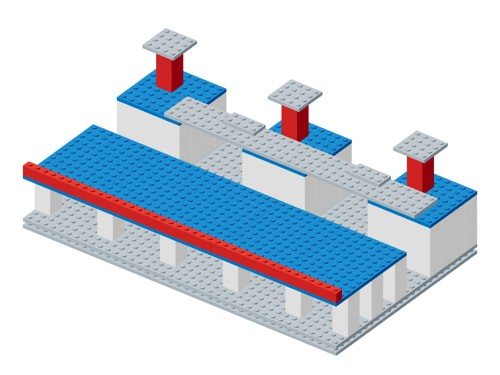
\includegraphics[width=.24\textwidth]{figures/frontier/process-service-plant-inspection-policy-good.jpg}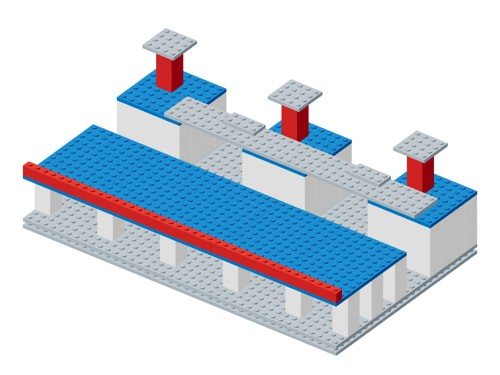
\includegraphics[width=.24\textwidth]{figures/frontier/process-service-plant-inspection-policy-bad.jpg}\hfill\begin{minipage}[b]{.48\textwidth}\small Positive success: 1. Negative success: 0.\\Rejection: \texttt{policy\_coverage\_or\_budget}.\\
Positive metrics: worldCoverage=1, worstCost=6.\end{minipage}\par
\noindent\small Positive policy queries q0, q1, q2 and identifies all eight worlds at worst cost 6; the negative guesses h0 without querying. Full branch tree is in the corresponding review JSON.\par\normalsize
\subsubsection*{distributed repair}
\noindent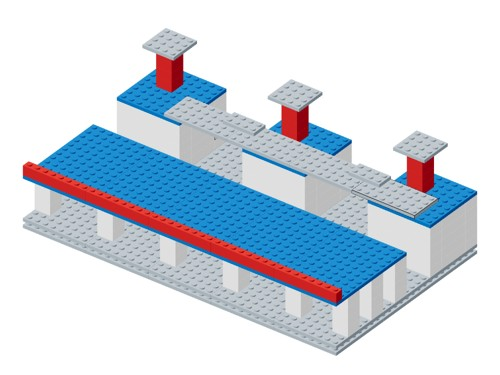
\includegraphics[width=.24\textwidth]{figures/frontier/process-service-plant-distributed-repair-good.jpg}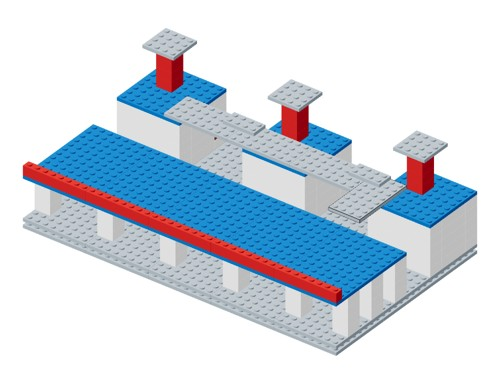
\includegraphics[width=.24\textwidth]{figures/frontier/process-service-plant-distributed-repair-bad.jpg}\hfill\begin{minipage}[b]{.48\textwidth}\small Positive success: 1. Negative success: 0.\\Rejection: \texttt{fault\_set}.\\
Positive metrics: finalExact=1, changedRecall=1.\end{minipage}\par
\clearpage
\subsection{Four-Storey Archive}
408 parts; 19 bottom-Y levels; dependency depth 19.
\subsubsection*{service plan}
\noindent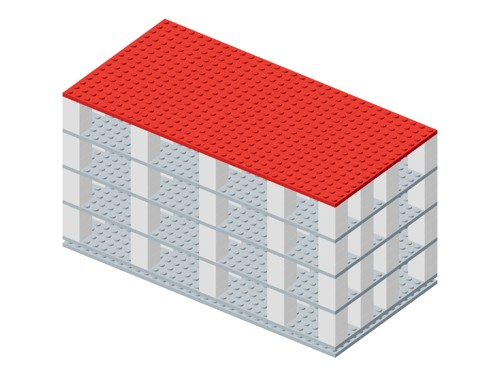
\includegraphics[width=.24\textwidth]{figures/frontier/four-storey-archive-service-plan-good.jpg}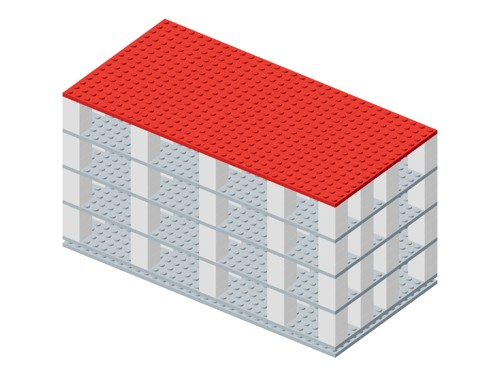
\includegraphics[width=.24\textwidth]{figures/frontier/four-storey-archive-service-plan-bad.jpg}\hfill\begin{minipage}[b]{.48\textwidth}\small Positive success: 1. Negative success: 0.\\Rejection: \texttt{blocked}.\\
Positive metrics: actions=50, lowerBound=50, finalExact=1, legalPrefix=1, excessActions=0.\end{minipage}\par
\subsubsection*{access certificate}
\noindent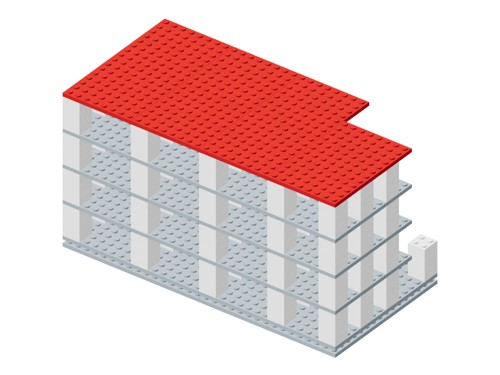
\includegraphics[width=.24\textwidth]{figures/frontier/four-storey-archive-access-certificate-good.jpg}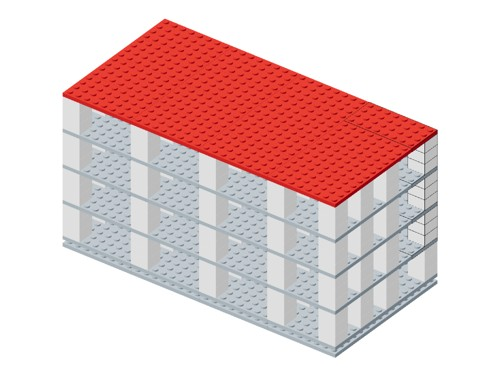
\includegraphics[width=.24\textwidth]{figures/frontier/four-storey-archive-access-certificate-bad.jpg}\hfill\begin{minipage}[b]{.48\textwidth}\small Positive success: 1. Negative success: 0.\\Rejection: \texttt{minimum\_set}.\\
Positive metrics: removals=25.\end{minipage}\par
\subsubsection*{parallel schedule}
\noindent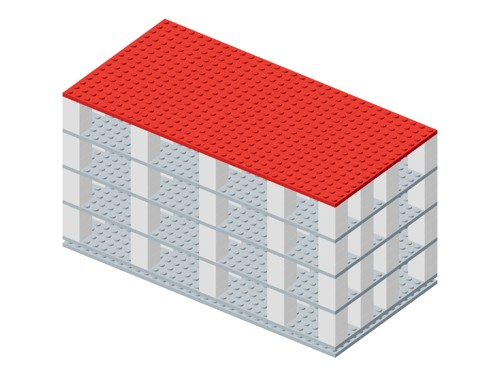
\includegraphics[width=.24\textwidth]{figures/frontier/four-storey-archive-parallel-schedule-good.jpg}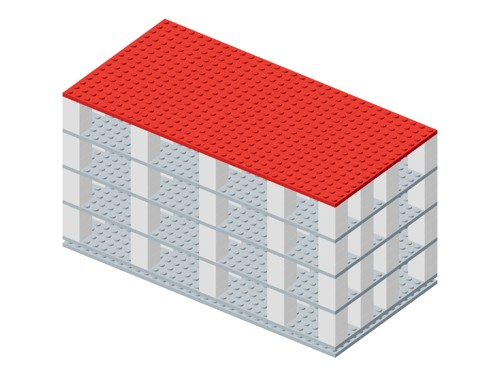
\includegraphics[width=.24\textwidth]{figures/frontier/four-storey-archive-parallel-schedule-bad.jpg}\hfill\begin{minipage}[b]{.48\textwidth}\small Positive success: 1. Negative success: 0.\\Rejection: \texttt{batch\_schema}.\\
Positive metrics: coverage=1, makespan=102, workerLowerBound=102.\end{minipage}\par
\subsubsection*{minimal intervention}
\noindent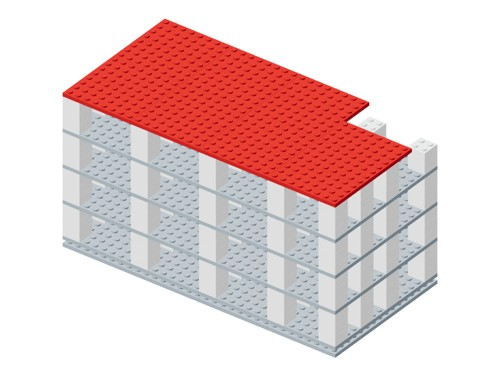
\includegraphics[width=.24\textwidth]{figures/frontier/four-storey-archive-minimal-intervention-good.jpg}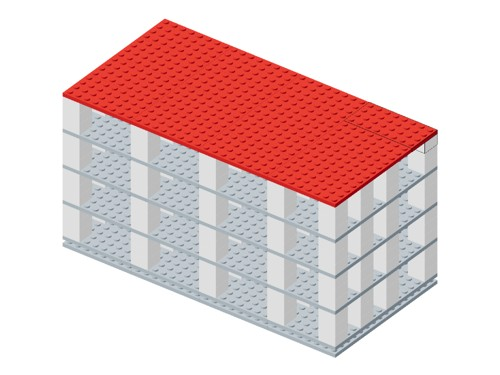
\includegraphics[width=.24\textwidth]{figures/frontier/four-storey-archive-minimal-intervention-bad.jpg}\hfill\begin{minipage}[b]{.48\textwidth}\small Positive success: 1. Negative success: 0.\\Rejection: \texttt{goal\_survives}.\\
Positive metrics: removals=2, optimum=2.\end{minipage}\par
\noindent\small\texttt{Positive: \{"removeIds": ["p0359", "p0371"], "cascadeIds": ["p0359", "p0371", "p0405"]\}}\par\normalsize
\clearpage
\subsection{Four-Storey Archive (continued)}
408 parts; 19 bottom-Y levels; dependency depth 19.
\subsubsection*{inventory cover}
\noindent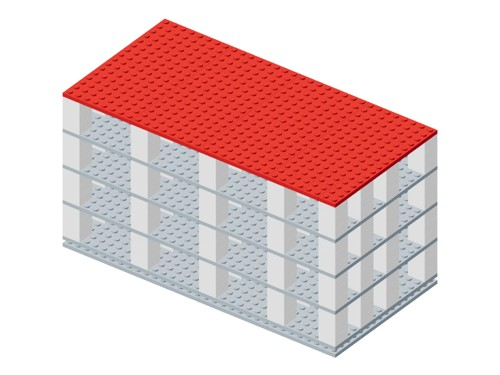
\includegraphics[width=.24\textwidth]{figures/frontier/four-storey-archive-inventory-cover-good.jpg}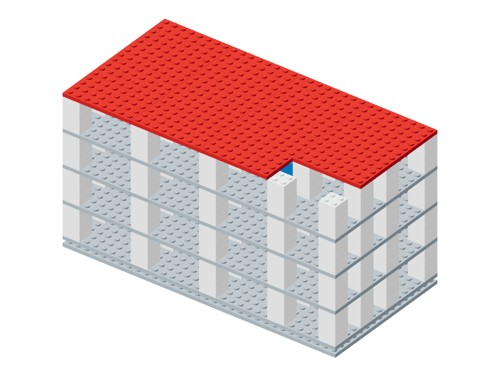
\includegraphics[width=.24\textwidth]{figures/frontier/four-storey-archive-inventory-cover-bad.jpg}\hfill\begin{minipage}[b]{.48\textwidth}\small Positive success: 1. Negative success: 0.\\Rejection: \texttt{uncovered}.\\
Positive metrics: coverage=1, tiles=7, lowerBound=7.\end{minipage}\par
\subsubsection*{ambiguity set}
\noindent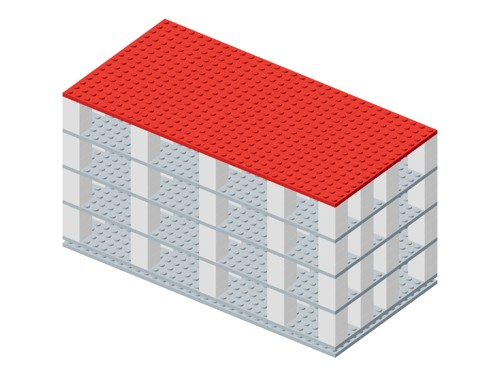
\includegraphics[width=.24\textwidth]{figures/frontier/four-storey-archive-ambiguity-set-good.jpg}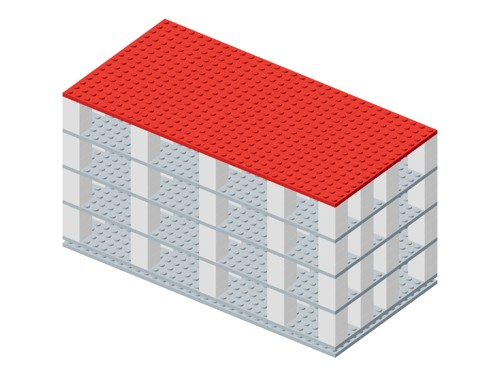
\includegraphics[width=.24\textwidth]{figures/frontier/four-storey-archive-ambiguity-set-bad.jpg}\hfill\begin{minipage}[b]{.48\textwidth}\small Positive success: 1. Negative success: 0.\\Rejection: \texttt{admissible\_set}.\\
Positive metrics: admissible=4, falseCertainty=0.\end{minipage}\par
\noindent\small\texttt{Positive: \{"possibleIds": ["h0", "h2", "h4", "h6"]\}}\par\normalsize
\subsubsection*{inspection policy}
\noindent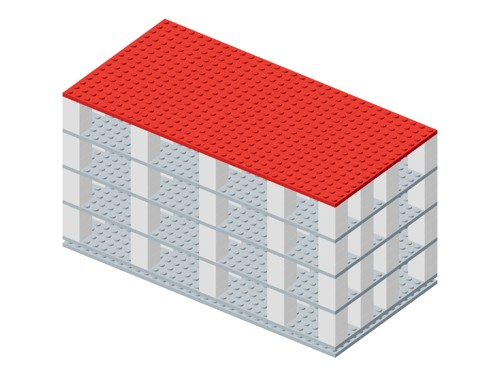
\includegraphics[width=.24\textwidth]{figures/frontier/four-storey-archive-inspection-policy-good.jpg}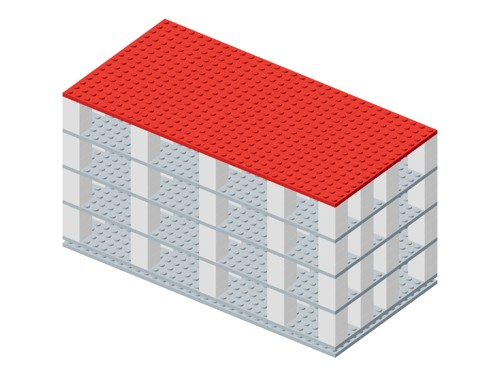
\includegraphics[width=.24\textwidth]{figures/frontier/four-storey-archive-inspection-policy-bad.jpg}\hfill\begin{minipage}[b]{.48\textwidth}\small Positive success: 1. Negative success: 0.\\Rejection: \texttt{policy\_coverage\_or\_budget}.\\
Positive metrics: worldCoverage=1, worstCost=6.\end{minipage}\par
\noindent\small Positive policy queries q0, q1, q2 and identifies all eight worlds at worst cost 6; the negative guesses h0 without querying. Full branch tree is in the corresponding review JSON.\par\normalsize
\subsubsection*{distributed repair}
\noindent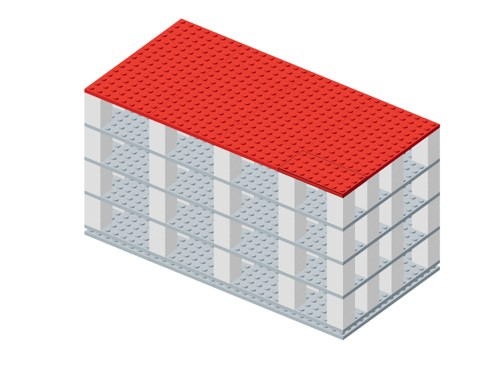
\includegraphics[width=.24\textwidth]{figures/frontier/four-storey-archive-distributed-repair-good.jpg}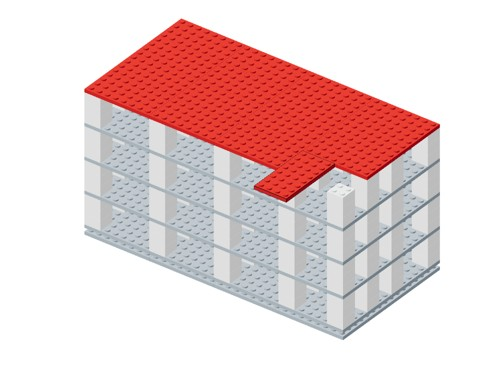
\includegraphics[width=.24\textwidth]{figures/frontier/four-storey-archive-distributed-repair-bad.jpg}\hfill\begin{minipage}[b]{.48\textwidth}\small Positive success: 1. Negative success: 0.\\Rejection: \texttt{fault\_set}.\\
Positive metrics: finalExact=1, changedRecall=1.\end{minipage}\par
